\documentclass[12pt]{article}
\usepackage[utf8]{inputenc}
\usepackage[dvips]{graphicx}
\usepackage{epsfig}
\usepackage{verbatim}
\usepackage{array}
\usepackage{latexsym}
\usepackage{hyperref}
\usepackage{listings}
\usepackage{color}
\usepackage[hmargin=3cm,vmargin=5.0cm]{geometry}

\usepackage{arydshln}
\usepackage{amssymb}
\usepackage[shortlabels]{enumitem}



\topmargin=-1.8cm
\addtolength{\textheight}{6.5cm}
\addtolength{\textwidth}{2.0cm}
\setlength{\oddsidemargin}{0.0cm}
\setlength{\evensidemargin}{0.0cm}

\newcommand{\HRule}{\rule{\linewidth}{1mm}}

\usepackage{tikz}
\usetikzlibrary{trees}
\tikzset{
  font={\fontsize{7pt}{12}\selectfont}}
  
\newcommand{\Q}{\raisebox{1.7pt}{$\scriptstyle\bigcirc$}}

\lstset{
    %backgroundcolor=\color{lbcolor},
    tabsize=2,
    language=C++,
    basicstyle=\footnotesize,
    numberstyle=\footnotesize,
    aboveskip={0.0\baselineskip},
    belowskip={0.0\baselineskip},
    columns=fixed,
    showstringspaces=false,
    breaklines=true,
    prebreak=\raisebox{0ex}[0ex][0ex]{\ensuremath{\hookleftarrow}},
    %frame=single,
    showtabs=false,
    showspaces=false,
    showstringspaces=false,
    identifierstyle=\ttfamily,
    keywordstyle=\color[rgb]{0,0,1},
    commentstyle=\color[rgb]{0.133,0.545,0.133},
    stringstyle=\color[rgb]{0.627,0.126,0.941},
}

\usepackage[]{mdframed}
\usepackage{enumitem}

\usepackage{titlesec}
\titleformat{\subsection}[runin]{}{}{}{}[]









\begin{document}

% Set the overall layout of the tree
\tikzstyle{level 1}=[level distance=2.5cm, sibling distance=20em]
\tikzstyle{level 2}=[level distance=2.5cm, sibling distance=10em]

% Define styles for bags and leafs
\tikzstyle{bag} = [text width=16em, text centered, align=center]
\tikzstyle{end} = [circle, minimum width=3pt,fill, inner sep=0pt]

\noindent
\HRule \\[3mm]
\small
\begin{tabular}[b]{lp{4.3cm}r}
Middle East Technical University &  &
Department of Computer Engineering \\
\end{tabular} \\
\begin{center}

                 \LARGE \textbf{CENG 280} \\[4mm]
                 \Large Formal Languages and Abstract Machines \\[4mm]
                \normalsize Spring 2022-2023 \\
                    \Large Homework 2 \\
\end{center}
\HRule



% Write down your name, surname, and student ID below.
\begin{center}
Name Surname: Berk Ulutaş  \\
Student ID: 2522084
\end{center}



\section*{Answer for Q1}

\subsection*{a.} 
$(a(b+c)^*a + b + aa)(a+b)^*$
 
\subsection*{b.}    \hfill\\
\textbf{A=}:  0      \newline
\textbf{B=}:  1      \newline
\textbf{C=}:  0,1      \newline
\textbf{D=}:   2     \newline
\textbf{E=}:    1    \newline
\textbf{F=}:   0,2     



\section*{Answer for Q2}
\subsection*{a.} 
The algorithm which is used for convert DFA/NFA to a Regular Expression (State elimination).
 \subsection*{b.} 
 \begin{itemize}
     \item Create a new starting state and connect it the previous starting state with empty transition. If machine do not read anything it cannot output anything.
     \item Create a final state and connect all states to the final state with empty transition. Empty transitions do not output anything. Since, the input can end in any state. all outputs will be in the language regardless of which state it ends in.
     \item After this modifications, we have an NFA-like machine. If we can treat (input/output) transitions to just like a normal transition. We can convert this NFA-like machine to a regular expression which gives the set of (input/output) strings in regular expression format that can be produced by a Mealy Machine. We can easily produce just set of output strings by ignoring inputs in (input/output).
 \end{itemize}

 \subsection*{c.} 
 Create two new states $q_s$ and $q_f$. Add empty transition from $q_s$ to $q_0$ and make $q_s$ new starting state. Create 'C' transition from $q_2$ to $q_f$ and make $q_f$ accepting state. \\

 
Step 1
\begin{center}
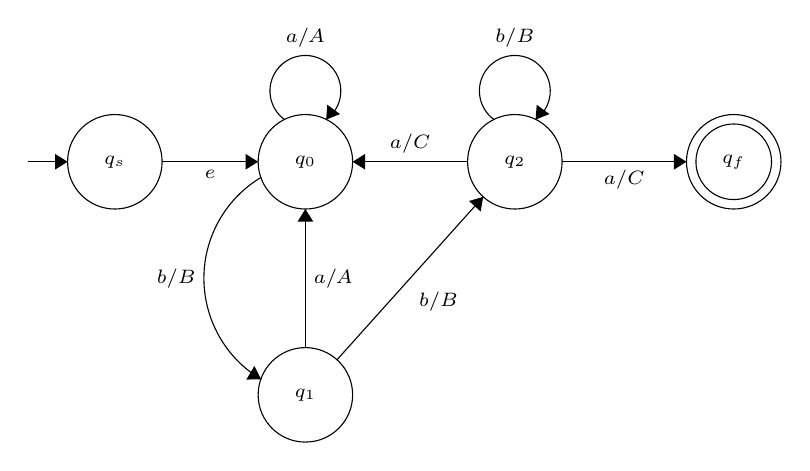
\begin{tikzpicture}[scale=0.2]
\tikzstyle{every node}+=[inner sep=0pt]
\draw [black] (12.7,-21.6) circle (3);
\draw (12.7,-21.6) node {$q_s$};
\draw [black] (52,-21.6) circle (3);
\draw (52,-21.6) node {$q_f$};
\draw [black] (52,-21.6) circle (2.4);
\draw [black] (24.8,-21.6) circle (3);
\draw (24.8,-21.6) node {$q_0$};
\draw [black] (24.8,-36.4) circle (3);
\draw (24.8,-36.4) node {$q_1$};
\draw [black] (38.1,-21.6) circle (3);
\draw (38.1,-21.6) node {$q_2$};
\draw [black] (41.1,-21.6) -- (49,-21.6);
\fill [black] (49,-21.6) -- (48.2,-21.1) -- (48.2,-22.1);
\draw (45.05,-22.1) node [below] {$a/C$};
\draw [black] (35.1,-21.6) -- (27.8,-21.6);
\fill [black] (27.8,-21.6) -- (28.6,-22.1) -- (28.6,-21.1);
\draw (31.45,-21.1) node [above] {$a/C$};
\draw [black] (15.7,-21.6) -- (21.8,-21.6);
\fill [black] (21.8,-21.6) -- (21,-21.1) -- (21,-22.1);
\draw (18.75,-22.1) node [below] {$e$};
\draw [black] (21.989,-35.41) arc (-120.90493:-239.09507:7.471);
\fill [black] (21.99,-35.41) -- (21.56,-34.57) -- (21.05,-35.43);
\draw (17.86,-29) node [left] {$b/B$};
\draw [black] (24.8,-33.4) -- (24.8,-24.6);
\fill [black] (24.8,-24.6) -- (24.3,-25.4) -- (25.3,-25.4);
\draw (25.3,-29) node [right] {$a/A$};
\draw [black] (26.81,-34.17) -- (36.09,-23.83);
\fill [black] (36.09,-23.83) -- (35.19,-24.09) -- (35.93,-24.76);
\draw (31.99,-30.46) node [right] {$b/B$};
\draw [black] (36.777,-18.92) arc (234:-54:2.25);
\draw (38.1,-14.35) node [above] {$b/B$};
\fill [black] (39.42,-18.92) -- (40.3,-18.57) -- (39.49,-17.98);
\draw [black] (23.477,-18.92) arc (234:-54:2.25);
\draw (24.8,-14.35) node [above] {$a/A$};
\fill [black] (26.12,-18.92) -- (27,-18.57) -- (26.19,-17.98);
\draw [black] (7.2,-21.6) -- (9.7,-21.6);
\fill [black] (9.7,-21.6) -- (8.9,-21.1) -- (8.9,-22.1);
\end{tikzpicture}
\end{center}

Step 2 eliminate $q_2$

\begin{center}
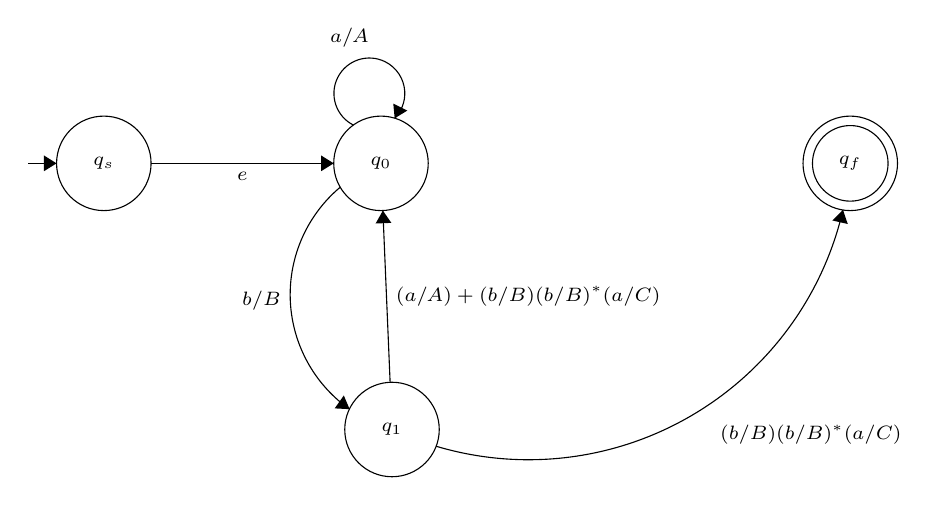
\begin{tikzpicture}[scale=0.2]
\tikzstyle{every node}+=[inner sep=0pt]
\draw [black] (11.8,-26.2) circle (3);
\draw (11.8,-26.2) node {$q_s$};
\draw [black] (29.4,-26.2) circle (3);
\draw (29.4,-26.2) node {$q_0$};
\draw [black] (59.2,-26.2) circle (3);
\draw (59.2,-26.2) node {$q_f$};
\draw [black] (59.2,-26.2) circle (2.4);
\draw [black] (30.1,-43.1) circle (3);
\draw (30.1,-43.1) node {$q_1$};
\draw [black] (7,-26.2) -- (8.8,-26.2);
\fill [black] (8.8,-26.2) -- (8,-25.7) -- (8,-26.7);
\draw [black] (14.8,-26.2) -- (26.4,-26.2);
\fill [black] (26.4,-26.2) -- (25.6,-25.7) -- (25.6,-26.7);
\draw (20.6,-26.7) node [below] {$e$};
\draw [black] (27.406,-41.812) arc (-125.19499:-230.06132:8.906);
\fill [black] (27.41,-41.81) -- (27.04,-40.94) -- (26.46,-41.76);
\draw (23.08,-34.92) node [left] {$b/B$};
\draw [black] (29.98,-40.1) -- (29.52,-29.2);
\fill [black] (29.52,-29.2) -- (29.06,-30.02) -- (30.06,-29.98);
\draw (30.31,-34.63) node [right] {$(a/A)+(b/B)(b/B)^*(a/C)$};
\draw [black] (27.656,-23.773) arc (243.42995:-44.57005:2.25);
\draw (27.4,-18.85) node [above] {$a/A$};
\fill [black] (30.27,-23.34) -- (31.07,-22.85) -- (30.18,-22.4);
\draw [black] (58.737,-29.161) arc (-13.08734:-106.62039:20.503);
\fill [black] (58.74,-29.16) -- (58.07,-29.83) -- (59.04,-30.05);
\draw (56.7,-42.76) node [below] {$(b/B)(b/B)^*(a/C)$};
\end{tikzpicture}
\end{center}

Step 3 eliminate $q_1$
\begin{center}
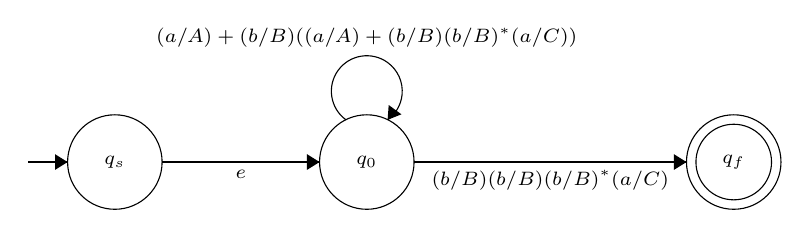
\begin{tikzpicture}[scale=0.2]
\tikzstyle{every node}+=[inner sep=0pt]
\draw [black] (12.7,-21.6) circle (3);
\draw (12.7,-21.6) node {$q_s$};
\draw [black] (52,-21.6) circle (3);
\draw (52,-21.6) node {$q_f$};
\draw [black] (52,-21.6) circle (2.4);
\draw [black] (28.7,-21.6) circle (3);
\draw (28.7,-21.6) node {$q_0$};
\draw [black] (15.7,-21.6) -- (25.7,-21.6);
\fill [black] (25.7,-21.6) -- (24.9,-21.1) -- (24.9,-22.1);
\draw (20.7,-22.1) node [below] {$e$};
\draw [black] (27.377,-18.92) arc (234:-54:2.25);
\draw (28.7,-14.35) node [above] {$(a/A) + (b/B)((a/A)+(b/B)(b/B)^*(a/C))$};
\fill [black] (30.02,-18.92) -- (30.9,-18.57) -- (30.09,-17.98);
\draw [black] (7.2,-21.6) -- (9.7,-21.6);
\fill [black] (9.7,-21.6) -- (8.9,-21.1) -- (8.9,-22.1);
\draw [black] (31.7,-21.6) -- (49,-21.6);
\fill [black] (49,-21.6) -- (48.2,-21.1) -- (48.2,-22.1);
\draw (40.35,-22.1) node [below] {$(b/B)(b/B)(b/B)^*(a/C)$};
\end{tikzpicture}
\end{center}

Step 4 eliminate $q_0$

\begin{center}
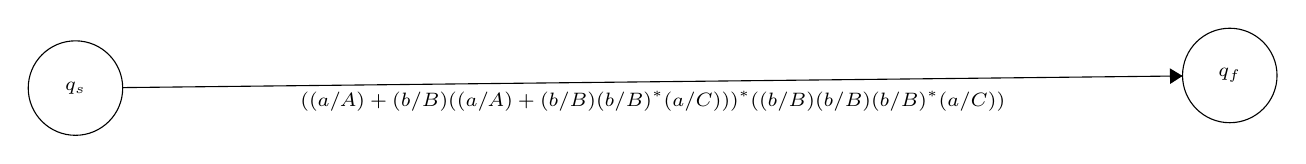
\begin{tikzpicture}[scale=0.2]
\tikzstyle{every node}+=[inner sep=0pt]
\draw [black] (3.4,-26.4) circle (3);
\draw (3.4,-26.4) node {$q_s$};
\draw [black] (76.7,-25.6) circle (3);
\draw (76.7,-25.6) node {$q_f$};
\draw [black] (6.4,-26.37) -- (73.7,-25.63);
\fill [black] (73.7,-25.63) -- (72.89,-25.14) -- (72.91,-26.14);
\draw (40.06,-26.57) node [below] {$((a/A) + (b/B)((a/A)+(b/B)(b/B)^*(a/C)))^*((b/B)(b/B)(b/B)^*(a/C))$};
\end{tikzpicture}
\end{center}

Set of output strings of $M_1$ which are ending
with C as a regular expression: $$(A+B(A+BB^*C))^*BBB^*C$$


\section*{Answer for Q3}
$P$ machine I/O is $[(a/A) + (b/B)(a/A) + (b/B)(b/B)(a/C)]^* + [(b/B)(b/B)]^*$. Let's analyze which input/output expression we can accept, and write a general regular expression for strings we can accept with $N_2$ or $N_3$.

Start with $N_2$ machine
\begin{itemize}
    \item We accept strings that can reach $q_2$ state. 
    \item $A^* $ or $ (BB)^*$ strings can be generated by $P$ machine and accepted by $N_2$ machine. 
    \item To generate $A^* $ or $ (BB)^*$ we need $(a)^* + (bb)^*$ as input. 
\end{itemize}

For $N_3$ machine
\begin{itemize}
    \item We accept strings that can reach $q_3$ state. To reach the $q_3$ state, it is necessary to be in the $q_0$ or $q_4$ state. However, a C output is required to reach $q_3$ while in q4.  This is not possible as the $P$ machine does not produce an output starting with C. In this case, we cannot reach from $q_4$ to $q_3$. 
    \item Now let's look at all the cases that can be produced by the machine $P$  which we can reach $q_0$ from the starting state. $(A + BBC)^*$ to generate this output we need $(a+bba)^*$ as a input.
    \item We need output B to go from state $q_0$ to $q_3$. Output B can be produced by machine $P$ in 2 ways either $(b/B)(a/A)$ or $(b/B)(b/B)(a/C)$. But we cannot go with $(b/B)(b/B)(a/C)$ case since there is no $C$ transition in $q_3$. In this case output should be $(A + BBC)^*(BA)$ to create this output we need $(a+bba)^*ba$ as input.
    \item We are now in the $q_3$ state of the $N_3$ machine. We can continue to stay in the $q_3$ state by taking the $(A+BA)^*$ output. $(a+ba)^*$ input is required to get this output.
    \item As a result, from the start $(A+BBC)^*BA(A+BA)^*$ output can be produced by machine $P$ and accepted by $N_3$. To produce this output we need $(a+bba)^*ba(a+ba)^*$ as input.
\end{itemize}

After all these steps the regular expression $a^* + (bb)^* + (a+bba)^*ba(a + ba)^*$  is inputs accepted by the whole machine. We can convert this regular expression to a DFA. First create a NFA from regular expression then convert it to a DFA.

\includegraphics[width=\textwidth]{imags/nfa.jpg} 

Since the steps of converting from NFA to DFA take too long, I could not draw all of them one by one. The latest version of DFA is below

\begin{center}
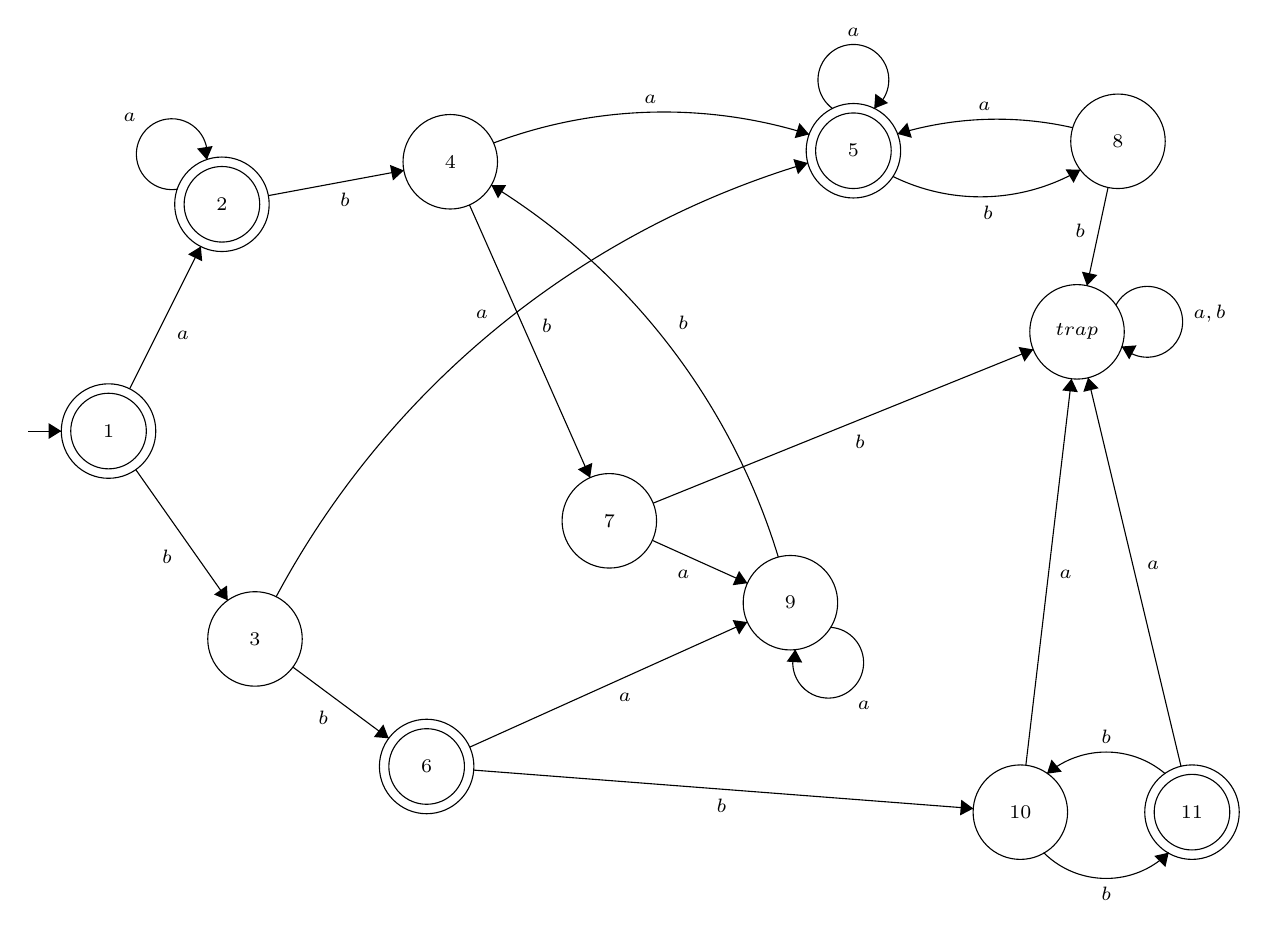
\begin{tikzpicture}[scale=0.2]
\tikzstyle{every node}+=[inner sep=0pt]
\draw [black] (5.7,-26.7) circle (3);
\draw (5.7,-26.7) node {$1$};
\draw [black] (5.7,-26.7) circle (2.4);
\draw [black] (12.9,-12.3) circle (3);
\draw (12.9,-12.3) node {$2$};
\draw [black] (12.9,-12.3) circle (2.4);
\draw [black] (15,-39.9) circle (3);
\draw (15,-39.9) node {$3$};
\draw [black] (27.4,-9.6) circle (3);
\draw (27.4,-9.6) node {$4$};
\draw [black] (53,-8.9) circle (3);
\draw (53,-8.9) node {$5$};
\draw [black] (53,-8.9) circle (2.4);
\draw [black] (69.8,-8.3) circle (3);
\draw (69.8,-8.3) node {$8$};
\draw [black] (37.5,-32.4) circle (3);
\draw (37.5,-32.4) node {$7$};
\draw [black] (49,-37.6) circle (3);
\draw (49,-37.6) node {$9$};
\draw [black] (25.9,-48) circle (3);
\draw (25.9,-48) node {$6$};
\draw [black] (25.9,-48) circle (2.4);
\draw [black] (63.6,-50.9) circle (3);
\draw (63.6,-50.9) node {$10$};
\draw [black] (74.5,-50.9) circle (3);
\draw (74.5,-50.9) node {$11$};
\draw [black] (74.5,-50.9) circle (2.4);
\draw [black] (67.2,-20.4) circle (3);
\draw (67.2,-20.4) node {$trap$};
\draw [black] (0.6,-26.7) -- (2.7,-26.7);
\fill [black] (2.7,-26.7) -- (1.9,-26.2) -- (1.9,-27.2);
\draw [black] (7.04,-24.02) -- (11.56,-14.98);
\fill [black] (11.56,-14.98) -- (10.75,-15.48) -- (11.65,-15.92);
\draw (10,-20.61) node [right] {$a$};
\draw [black] (15.85,-11.75) -- (24.45,-10.15);
\fill [black] (24.45,-10.15) -- (23.57,-9.8) -- (23.76,-10.79);
\draw (20.72,-11.55) node [below] {$b$};
\draw [black] (7.43,-29.15) -- (13.27,-37.45);
\fill [black] (13.27,-37.45) -- (13.22,-36.51) -- (12.4,-37.08);
\draw (9.76,-34.67) node [left] {$b$};
\draw [black] (10.07,-11.34) arc (279:-9:2.25);
\draw (7.04,-7.05) node [above] {$a$};
\fill [black] (11.94,-9.47) -- (12.31,-8.6) -- (11.32,-8.76);
\draw [black] (16.345,-37.219) arc (151.84686:106.56755:56.59);
\fill [black] (50.1,-9.68) -- (49.19,-9.43) -- (49.48,-10.39);
\draw (29.4,-19.58) node [above] {$a$};
\draw [black] (17.41,-41.69) -- (23.49,-46.21);
\fill [black] (23.49,-46.21) -- (23.15,-45.33) -- (22.55,-46.13);
\draw (19.33,-44.45) node [below] {$b$};
\draw [black] (30.151,-8.407) arc (110.63586:72.49672:30.674);
\fill [black] (50.19,-7.86) -- (49.57,-7.14) -- (49.27,-8.1);
\draw (40.11,-5.92) node [above] {$a$};
\draw [black] (28.62,-12.34) -- (36.28,-29.66);
\fill [black] (36.28,-29.66) -- (36.42,-28.72) -- (35.5,-29.13);
\draw (33.18,-20.01) node [right] {$b$};
\draw [black] (51.677,-6.22) arc (234:-54:2.25);
\draw (53,-1.65) node [above] {$a$};
\fill [black] (54.32,-6.22) -- (55.2,-5.87) -- (54.39,-5.28);
\draw [black] (67.414,-10.107) arc (-59.68517:-116.22402:12.577);
\fill [black] (67.41,-10.11) -- (66.47,-10.08) -- (66.98,-10.94);
\draw (61.54,-12.36) node [below] {$b$};
\draw [black] (28.64,-46.77) -- (46.26,-38.83);
\fill [black] (46.26,-38.83) -- (45.33,-38.7) -- (45.74,-39.62);
\draw (38.49,-43.31) node [below] {$a$};
\draw [black] (28.89,-48.23) -- (60.61,-50.67);
\fill [black] (60.61,-50.67) -- (59.85,-50.11) -- (59.77,-51.11);
\draw (44.62,-50.03) node [below] {$b$};
\draw [black] (40.23,-33.64) -- (46.27,-36.36);
\fill [black] (46.27,-36.36) -- (45.74,-35.58) -- (45.33,-36.49);
\draw (42.21,-35.51) node [below] {$a$};
\draw [black] (30.008,-11.082) arc (58.36062:16.93462:42.172);
\fill [black] (30.01,-11.08) -- (30.43,-11.93) -- (30.95,-11.08);
\draw (41.85,-19.82) node [right] {$b$};
\draw [black] (69.666,-18.712) arc (152.1301:-135.8699:2.25);
\draw (74.57,-19.27) node [right] {$a,b$};
\fill [black] (70.04,-21.33) -- (70.51,-22.15) -- (70.98,-21.26);
\draw [black] (51.547,-39.163) arc (86.19652:-201.80348:2.25);
\draw (53.66,-43.81) node [below] {$a$};
\fill [black] (49.31,-40.57) -- (48.76,-41.34) -- (49.75,-41.4);
\draw [black] (73.023,-53.47) arc (-45.14762:-134.85238:5.633);
\fill [black] (73.02,-53.47) -- (72.1,-53.68) -- (72.81,-54.39);
\draw (69.05,-55.61) node [below] {$b$};
\draw [black] (65.293,-48.464) arc (130.37762:49.62238:5.799);
\fill [black] (65.29,-48.46) -- (66.23,-48.33) -- (65.58,-47.56);
\draw (69.05,-46.58) node [above] {$b$};
\draw [black] (55.801,-7.833) arc (106.88902:77.2018:21.733);
\fill [black] (55.8,-7.83) -- (56.71,-8.08) -- (56.42,-7.12);
\draw (61.31,-6.37) node [above] {$a$};
\draw [black] (40.28,-31.28) -- (64.42,-21.52);
\fill [black] (64.42,-21.52) -- (63.49,-21.36) -- (63.86,-22.29);
\draw (53.42,-26.92) node [below] {$b$};
\draw [black] (63.95,-47.92) -- (66.85,-23.38);
\fill [black] (66.85,-23.38) -- (66.26,-24.12) -- (67.25,-24.23);
\draw (66.06,-35.77) node [right] {$a$};
\draw [black] (73.8,-47.98) -- (67.9,-23.32);
\fill [black] (67.9,-23.32) -- (67.6,-24.21) -- (68.57,-23.98);
\draw (71.61,-35.22) node [right] {$a$};
\draw [black] (69.17,-11.23) -- (67.83,-17.47);
\fill [black] (67.83,-17.47) -- (68.49,-16.79) -- (67.51,-16.58);
\draw (67.75,-13.99) node [left] {$b$};
\end{tikzpicture}
\end{center}



\end{document}

